%% Direttive TeXworks:
% !TeX root = ../../presentazione.tex
% !TEX encoding = UTF-8 Unicode
% !TEX program = arara
% !TEX TS-program = arara
% !TeX spellcheck = it-IT

\section{Introduzione}\label{sec:intro}
\begin{frame}
    \frametitle{\insertsection}

    Lo scopo di questa tesi è la progettazione e la successiva implementazione di un'interfaccia grafica 2D per il simulatore \emph{Alchemist}.

    \medskip % non soono sicuro sia la soluzione più corretta, am funziona
    \pause

    La nuova interfaccia permette di interagire con la simulazione a tempo di esecuzione e di vedere chiaramente rappresentate informazioni su di essa.
\end{frame}

\begin{frame}
    \frametitle{\insertsection}

    In particolare, è supportata una \emph{struttura modulare di effetti} che rende facilmente osservabili determinate entità del sistema ed eventuali loro proprietà:

    \begin{itemize}[<+(1)->]
        \item
            l'effetto non fa più riferimento al singolo nodo, bensì costituisce una funzione dall'intero ambiente alla rappresentazione grafica.
        \item
            gli \engEmph{stack} di effetti realizzati possono essere serializzati su file di testo in formato JSON.
    \end{itemize}
\end{frame}

\begin{frame}
    \frametitle{\insertsection}

    Si è scelto di mantenere un'interfaccia il più possibile \engEmph{user-friendly}, mantenendo un design più simile ai simulatori a scopo videoludico per favorire l'utilizzo da parte di utenti inesperti.

    \medskip
    \pause

    Lo stile estetico al quale si è deciso di allinearsi è il \emph{Material Design} di Google\only<2->{\footnote{\url{https://material.io}}} e la libreria grafica utilizzata per l'implementazione è stata \emph{JavaFX}.
\end{frame}

\section{Alchemist}\label{sec:alchemist}

\subsection{Introduzione ad Alchemist}\label{subsec:alchIntro}
\begin{frame}
    \frametitle{\insertsection}
    \framesubtitle{\insertsubsection}

    Alchemist\only<1->{\footnote{\url{http://alchemistsimulator.github.io}}} è un meta-simulatore estendibile completamente open-source che esegue su Java Virtual Machine (JVM), nato all’interno dell’Università di Bologna e reperibile su GitHub\only<1->{\footnote{\url{https://github.com/AlchemistSimulator/Alchemist}}}.

    \medskip
    \pause

    L'idea dietro al progetto è quello di riuscire ad avere un framework di simulazione il più possibile generico, in grado di simulare sistemi di tipologia e complessità diverse, mantenendo le prestazioni dei simulatori non generici (come ad esempio quelli impiegati in ambito chimico.
\end{frame}

\subsection{Il modello di Alchemist}\label{subsec:alchModel}
\begin{frame}
    \frametitle{\insertsection}
    \framesubtitle{\insertsubsection}

    \centering
    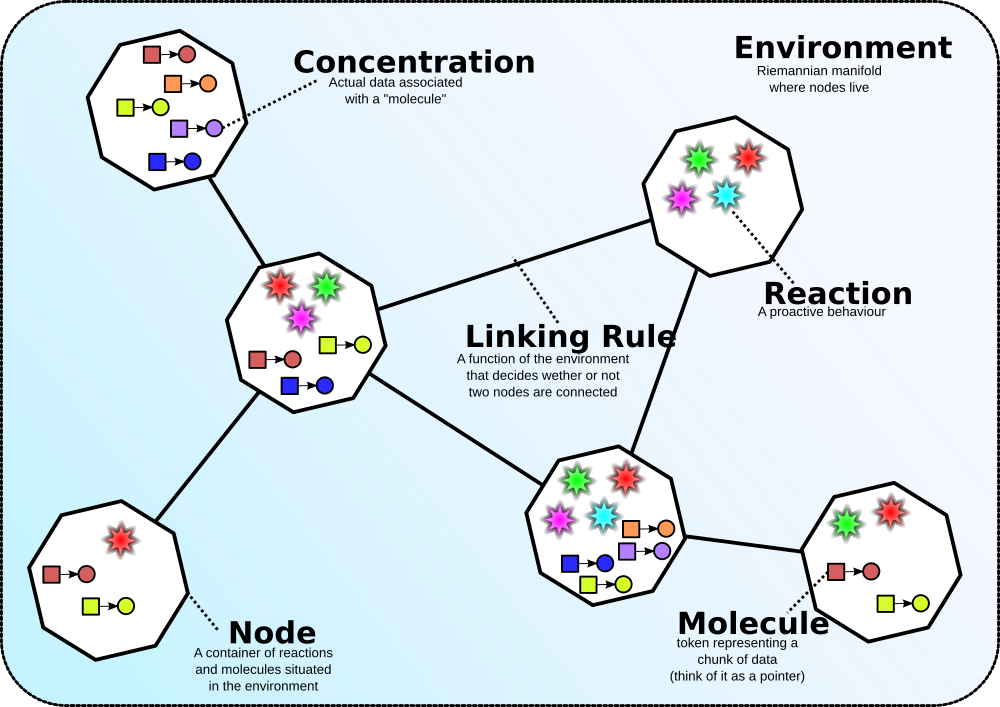
\includegraphics[scale=.34]{fig/alchemist_model}
\end{frame}

\begin{frame}
    \frametitle{\insertsection}
    \framesubtitle{\insertsubsection}

    \begin{description}[<+->]
        \item[Molecola]\label{itm:mol}
            Una \emph{Molecola} rappresenta il nome dato ad un particolare dato all'interno di un \emph{Nodo}, del quale ne astrae parte dello stato.

        \item[Concentrazione]\label{itm:conc}
            La \emph{Concentrazione} di una \emph{Molecola} è il valore associato alla proprietà rappresentata dalla \emph{Molecola}.

        \item[Nodo]\label{itm:node}
            Il \emph{Nodo} è un contenitore di \emph{Molecole} e \emph{Reazioni} che risiede all'interno di un \emph{Ambiente} e che astrae una singola entità.

        \item[Ambiente]\label{itm:env}
            L'\emph{Ambiente} è l'astrazione che rappresenta lo spazio nella simulazione ed è l'entità che contiene i \emph{Nodi}.

        \item[Regola di collegamento]\label{itm:linkr}
            La \emph{Regola di collegamento} è una funzione dello stato corrente dell'\emph{Ambiente} che associa ad ogni \emph{Nodo} un \emph{Vicinato}.
    \end{description}
\end{frame}

\begin{frame}
    \frametitle{\insertsection}
    \framesubtitle{\insertsubsection}

    \begin{description}[<+->]
        \item[Vicinato]\label{itm:neigh}
            Un \emph{Vicinato} è un'entità costituita da un \emph{Nodo} detto ``centro'' e da un insieme di altri \emph{Nodi} (i ``vicini'').

        \item[Reazione]\label{itm:react}
            Una \emph{Reazione} è un insieme di \emph{Condizioni} sullo stato del sistema che qualora dovessero risultare vere innescherebbero l'esecuzione di un insieme di \emph{Azioni}.

            Ogni \emph{Nodo} è costituito da un insieme (anche vuoto) di \emph{Reazioni}.

        \item[Condizione]\label{itm:cond}
            Una \emph{Condizione} è una funzione che associa un valore numerico e un valore booleano allo stato corrente di un \emph{Ambiente}.

        \item[Azione]\label{itm:act}
            Un'\emph{Azione} è una procedura che provoca una modifica allo stato dell'\emph{Ambiente}.
    \end{description}
\end{frame}
